% Trabalho de Gradua��o Interdisciplinar - Christian Hartung
\documentclass[times]{abnt}

\usepackage[brazil]{babel}
\usepackage[latin1]{inputenc}
\usepackage[T1]{fontenc}
\usepackage{color}
\usepackage{graphics}
\usepackage[pdftex]{graphicx}
\usepackage{float}
\usepackage{booktabs}
\usepackage{mdwlist}
\usepackage{listings}
\usepackage{booktabs}
\usepackage[num]{abntcite}

% A grossura padr�o da linha de assinatura � 0. Aumento para 0.4, s� para ela aparecer
\setlength{\ABNTsignthickness}{0.4pt}
\setlength{\ABNTsignskip}{2cm}
\setlength{\ABNTsignwidth}{6.5cm}

% Configura��es da package listings
\lstset{ %
basicstyle=\footnotesize,       % the size of the fonts that are used for the code
numbers=left,                   % where to put the line-numbers
numberstyle=\footnotesize,      % the size of the fonts that are used for the line-numbers
stepnumber=1,                   % the step between two line-numbers. If it's 1, each line 
                                % will be numbered
numbersep=6pt,                  % how far the line-numbers are from the code
backgroundcolor=\color{white},  % choose the background color. You must add \usepackage{color}
showspaces=false,               % show spaces adding particular underscores
showstringspaces=false,         % underline spaces within strings
showtabs=false,                 % show tabs within strings adding particular underscores
tabsize=2,                      % sets default tabsize to 2 spaces
captionpos=b,                   % sets the caption-position to bottom
breaklines=true,                % sets automatic line breaking
breakatwhitespace=false,        % sets if automatic breaks should only happen at whitespace
escapeinside={\%*}{*)},         % if you want to add a comment within your code
frame=single,                   % adds a frame around the code
}

\autor{Christian Hartung}
\titulo{Detec��o de Vulnerabilidades XPath Injection em Web Services}
\comentario{Trabalho de Gradua��o Interdisciplinar apresentado na Faculdade de Tecnologia - FT como requisito de conclus�o do curso de Tecnologia em An�lise e Desenvolvimento de Sistemas.}
\instituicao{Universidade Estadual de Campinas - UNICAMP\par
 Faculdade de Tecnologia - FT}
\orientador[Orientadora:]{\small Prof. Tania Basso}
\coorientador[Co-orientadora:]{\small Prof. Dr. Regina L. O. Moraes}
\local{Limeira}
\data{2011}

\begin{document}
\capa
\folhaderosto

% Errata

% Dedicat�ria

% Agradecimentos

% Ep�grafe

\sumario

\listoffigures

\listoftables

\pretextualchapter{Lista de siglas, abreviaturas e s�mbolos}
\begin{description*}
  \item[REST] \textit{Representational State Transfer} - Transfer�ncia de Estado Representacional
  \item[HTTP] \textit{Hypertext Transfer Protocol} - Protocolo de Transferencia de Hipertexto
  \item[API] \textit{Application Programming Interface} - Interface de Programa��o de Aplica��es
  \item[RPC] \textit{Remote Procedure Call} - Chamada Remota de Procedimento
  \item[SOAP] \textit{Simple Object Access Protocol} - Protocolo Simples de Acesso a Objetos
  \item[XML] \textit{Extensible Markup Language} - Linguagem de Marca��o Extens�vel
  \item[WSDL] \textit{Web Services Description Language} - Linguagem de Descri��o de Servi�os Web
\end{description*}

\begin{resumo}
 Servi�os web podem apresentar vulnerabilidades de seguran�a. Scanners de vulnerabilidades s�o ferramentas capazes de detectar vulnerabilidades de seguran�a em servi�os web. O objetivo do trabalho � avaliar a seguran�a de servi�os web em rela��o � vulnerabilidade do tipo \emph{XPath Injection} e tamb�m avaliar a efic�cia de scanners de vulnerabilidades na detec��o dessas vulnerabilidades.
\end{resumo}

\chapter{Web Services}
Nos �ltimos anos, muito se tem falado sobre as vantagens de se utilizar a chamada \textit{cloud computing} (computa��o em nuvem) como arquitetura de TI.

Essa arquitetura permite que as aplica��es fiquem armazenadas em centros de armazenamento de terceiros\cite{Silva-Fabio-Rodrigues:2010:CloudComputing}, e sejam acessadas das m�quinas clientes, reduzindo assim os custos com compra e manuten��o de servidores, dispositivos para armazenamento, backups, etc. Apenas o acesso ao servi�o � pago.

De forma resumida, ao inv�s de instalar um editor de textos na m�quina, ele funciona como um servi�o armazenado no provedor e existe uma interface para acess�-lo. Todos os recursos de hardware necess�rios para rod�-lo, o espa�o para armazenamento de documentos, etc. ficam no provedor e � tudo feito via navegador de internet.

No lado pessoal, sites como Twitter e Facebook vem ganhando muita popularidade, principalmente pelo fato que os dados desses sites podem ser acessados em qualquer plataforma, sem nem precisar abrir o site.

Em ambos os casos � necess�ria comunica��o entre o dispositivo local e o servi�o remoto. Essa comunica��o � feita atrav�s dos chamados web services (servi�os web).

\section{Funcionamento}
Para que um web servisse funcione, dois componentes s�o necess�rios: os servidores, que armazenam os dados e podem realizar opera��es sobre eles, e os clientes, que s�o os dispositivos que solicitam que essas opera��es sejam realizadas.

\begin{figure}[H]
\centering
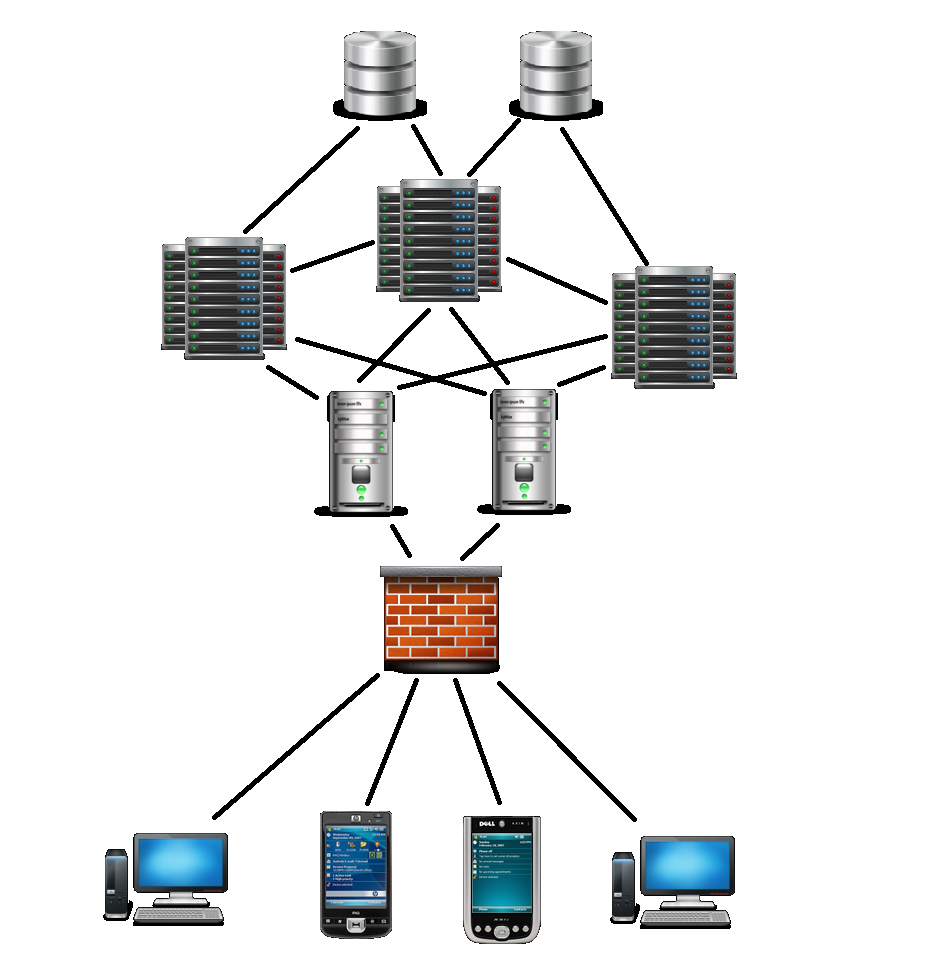
\includegraphics[width=7cm]{img/WebServices}%
\caption{Arquitetura de um web service}%
\label{fig:WebServices}%
\end{figure}

Na figura \ref{fig:WebServices}, podemos observar como � a arquitetura de um web service que pode ser considerado robusto. Nela, temos os dispositivos clientes (celulares, desktops, workstation) que se conectam ao provedor do servi�o. L� normalmente as chamadas passam por um firewall, que verifica se a porta que limita o acesso aos servidores onde o servi�o est� em execu��o, permitindo que apenas determinadas portas sejam acessadas. Ent�o a requisi��o vai para os servidores proxy, respons�veis por balancear a carga. O proxy encaminha a requisi��o para um servidor que estiver menos ocupado e ele acessa a base de dados buscando o recurso solicitado. Feito isso, o resultado do processamento � enviado para o cliente que o solicitou.

Para que ambas as partes possam se entender, elas devem conseguir se comunicar utilizando uma linguagem comum. A linguagem mais comum utilizada em web services � o XML\cite{Costa-Guilherme:2009:SOA}, uma linguagem de marca��o padronizada pela W3C\cite{W3C:XML}, que a define como um formato para representar informa��es estruturadas na forma de texto. Sua ado��o se d� principalmente por ele j� ter sido criado pensando em internet, em facilidade de uso, em ser independente de linguagem ou plataforma e em ser leg�vel, tanto para m�quinas como para humanos.

Estruturalmente falando, s�o documentos compostos por tags e atributos.	As tags s�o elementos envolvidos por \texttt{<>}, utilizados para expor informa��es, e os atributos s�o metadados dessas informa��es. Assim:
\begin{lstlisting}[language=XML]
<exemplo>
  <documento autor="Christian Hartung">Exemplo de documento XML</documento>
</exemplo>
\end{lstlisting}
\textit{exemplo} e \textit{documento} s�o tags. \textit{autor} � um atributo de \textit{documento}.

\section{SOAP}
O SOAP � um protocolo para troca de informa��es atrav�s da troca de mensagens XML sobre um protocolo de aplica��o, normalmente o HTTP. O SOAP � uma recomenda��o da W3C\cite{W3C:SOAP} desde 2003.

O SOAP tamb�m � um dos protocolos mais utilizados para cria��o de web services, principalmente pelo fato de ser aberto e ser baseado em XML, o que o torna compat�vel com qualquer linguagem de programa��o.

Funciona da seguinte forma: quando o cliente se conecta ao servi�o, obt�m um documento listando os m�todos dispon�veis, seus par�metros e tipos de dados. Este documento � chamado WSDL, uma linguagem tambem baseada em XML. A descri��o de uma mensagem para obter os dados de uma cidade seria:
\begin{lstlisting}[language=XML]
<wsdl:message name="GetCidade">
  <wsdl:part name="Cidade" type="xsd:string" />
</wsdl:message>
\end{lstlisting}
Neste trecho � especificado um m�todo getCidade, que recebe uma string como par�metro.

A resposta, uma string descrevendo a cidade, pode ser definida com a seguinte mensagem:
\begin{lstlisting}[language=XML]
<wsdl:message name="GetCidadeResponse">
 <wsdl:part name="GetCidadeReturn" type="xsd:string" />
</wsdl:message>
\end{lstlisting}

Tento este documento, o aplicativo cliente � capaz de fazer a requisi��o SOAP propriamente dita, enviando uma mensagem HTTP no seguinte formato:
\begin{lstlisting}[language=XML]
<?xml version="1.0"?>
<soap:Envelope xmlns:soap="http://www.w3.org/2003/05/soap-envelope">
  <soap:Header>
  </soap:Header>
  <soap:Body>
    <m:GetCidade xmlns:m="http://www.ft.unicamp.br/tgi">
      <m:Cidade>Limeira</m:Cidade>
    </m:GetCidade>
  </soap:Body>
</soap:Envelope>
\end{lstlisting}

\section{Vantagens e Desvantagens}
Utilizando web services, � poss�vel dividir o processamento que uma aplica��o precisa realizar entre os clientes e o servidor, tornando os aplicativos mais leves entre ambas as partes.

Por serem baseados em padr�es abertos, a grande maioria das linguagens de programa��o possui suas API's para cria��o de web services, e estas s�o compat�veis entre si, portanto o cliente e o servidor podem ser escritos em linguagens diferentes.

Um problema dessas tecnologias � que o XML pode ser considerado um formato pesado para troca de informa��es, j� que existe um conjunto de regras que devem ser seguidas, principalmente para garantir a compatibilidade.

Outra preocupa��o que se deve ter � com como os dados trafegar�o. Como o uso de web services envolve rede, ou mesmo a internet, � preciso que as requisi��es sejam criptografadas para evitar que os dados sejam obtidos por outros.
\chapter{XPath e XPath Injection} \label{chap:XPath}
A maioria das aplica��es web utilizam sistemas gerenciadores de bancos de dados (SGBD) para armazenar seus dados\cite{devWorks:XPath}, especialmente porque esses sistemas ajudam a garantir a integridade e facilitam a manipula��o das informa��es armazenadas. Por�m, utilizar um SGBD nem sempre � a melhor solu��o. Manter um SGBD n�o � uma tarefa barata. � preciso um especialista em cada SGBD utilizado, monitoramento constante, aquisi��o de servidores e at� mesmo licen�as de uso desses sistemas, etc. Para uma aplica��o pequena, por exemplo, um  esses gastos n�o compensariam. Tamb�m, se alguma customiza��o for feita para um caso espec�fico, n�o compensaria alterar a estrutura da base de dados da aplica��o para contemplar esse �nico caso. Para esses tipos de situa��es, documentos XML se tornam uma op��o interessante, com a vantagem de serem leg�veis para a aplica��o e para seus usu�rios e desenvolvedores.

\section{Entendendo o XPath}
A XML Path Language, ou XPath, como � mais conhecida, � uma linguagem de consulta capaz de localizar elementos de um documento XML e at� mesmo realizar c�lculos com esses elementos\cite{W3C:XPath}.

Em uma consulta XPath, o documento XML � visto como uma �rvore, onde cada tag, cada atributo, cada texto, cada coment�rio, etc. � tratado como um n�\cite{W3Schools:XPath}. A linguagem XPath permite navegar por essa �rvore, selecionando um conjunto de n�s baseado em uma s�rie de crit�rios. Desde 1999, XPath � uma recomenda��o da W3C\cite{W3C:XPath}. Suas principais express�es s�o:
\begin{description*}
  \item[\textit{nome}] - Seleciona todos os filhos com o nome dado
  \item[/] - Seleciona a partir do n� atual
  \item[//] - Seleciona todos os n�s do documento que satisfa�am o crit�rio, partindo do atual
  \item[.] - Seleciona o n� atual
  \item[..] - Seleciona o pai do n� atual
  \item[@] - Seleciona um atributo
\end{description*}

Considere o documento XML da figura \ref{fig:ExemploXPath}, extra�do de uma aplica��o real. Este documento � utilizado para controlar a aprova��o de cota��es de compra em um sistema ERP (\estrangeiro{Enterprise Resource Planning}, sistemas integrados de gest�o empresarial), baseando-se no valor da cota��o. Cada elemento VALOR lista os logins dos usu�rios que podem aprovar cota��es com valores iguais ou inferiores ao definido valor pelo atributo VALUE. No caso, o usu�rio EMILY pode aprovar cota��es de at� R\$500, o usu�rio TANIA pode aprovar cota��es de at� R\$999 e o usu�rio CHRISTIAN  pode aprovar cota��es de at� R\$1.000.000.

\figura{ExemploXPath}{Documento XML de exemplo para consultas}{7cm}

A seguir est�o algumas das principais express�es XPath aplicadas ao documento XML da figura \ref{fig:ExemploXPath}, junto de seus resultados:
\begin{description*}
  \item[VALCOMPRAS]\hfill \\
    Seleciona todos os filhos do elemento raiz (VALCOMPRAS)
  \item[/VALCOMPRAS]\hfill \\
    Seleciona o elemento raiz
  \item[VALCOMPRAS/VALOR]\hfill \\
    Seleciona todos os elementos VALOR filhos diretos de VALCOMPRAS
  \item[VALCOMPRAS//USER]\hfill \\
    Seleciona todos os elementos USER descendentes de VALCOMPRAS. N�o � necess�rio ser um filho direto
  \item[//@VALUE]\hfill \\
    Seleciona todos os atributos VALUE do documento
\end{description*}
Observe que as express�es s�o utilizadas para criar caminhos atrav�s do documento XML, da� o nome \textit{XML Path Language} (Linguagem de Caminhos pelo documento XML).

Para tornar o caminho at� determinado elemento mais espec�fico, � poss�vel filtrar as express�es. A seguir est�o alguns exemplos de filtros (express�es entre colchetes) aplicados ao documento da figura \ref{fig:ExemploXPath} e o resultado da consulta.
\begin{description*}
  \item[VALCOMPRAS/VALOR[1]]\hfill \\
    Seleciona o primeiro elemento VALOR filho de VALCOMPRAS
  \item[VALCOMPRAS/VALOR[last()]]\hfill \\
    Seleciona o �ltimo elemento VALOR filho de VALCOMPRAS
  \item[VALCOMPRAS/VALOR[position() <= 2]]\hfill \\
    Seleciona os dois primeiros elementos VALOR filhos de VALCOMPRAS
  \item[//VALOR[@VALUE]]\hfill \\
    Seleciona todos os elementos VALOR que possuam um atributo VALUE
  \item[//USERS[USER]]\hfill \\
    Seleciona todos os elementos USERS que tenham uma tag USER como filho
  \item[VALCOMPRAS/VALOR[@VALUE >= 1000]//USER]\hfill \\
    Seleciona todos os elementos USER que descendentes de um elemento VALOR com o atributo VALUE maior ou igual a 1000
  \item[//VALOR[@VALUE < 100 or @VALUE > 500]]\hfill \\
    Seleciona todos os elementos VALOR que tenham o elemento VALUE menor que 100 ou maior que 500
\end{description*}

\section{XPath Injection}
Segundo \cite{WASC:XPath}, XPath Injection � uma t�cnica para explorar aplica��es que montam consultas XPath a partir de dados fornecidos pelo usu�rio. � uma forma de vulnerabilidade de inje��o de c�digo.

O c�digo na figura \ref{fig:ExemploCSharp}, escrito em C\#, mostra uma aplica��o que consulta o documento XML da figura \ref{fig:ExemploXPath} para obter uma lista com todos os usu�rios que podem aprovar cota��es de compra de um determinado valor.

\figura{ExemploCSharp}{C�digo C\# executando uma consulta XPath}{13cm}

Na linha 3 � feita a consulta XPath baseando-se no valor de um campo de entrada. Supondo que a cota��o de compras seja de R\$1000, essa consulta ficaria ``\texttt{//VALOR[@VALUE >= 1000]/USERS/USER/@NAME}'' o que retorna a lista de nomes corretamente.

Como n�o existe nenhuma valida��o deste campo antes de seu uso, o usu�rio pode informar qualquer conte�do para este campo. Por exemplo, se o par�metro tiver o formato 1000 or 1 = 1, a consulta ficaria ``\texttt{//VALOR[@VALUE >= 1000 or 1 = 1]/USERS/USER/@NAME}'' retornando os nomes de todos os usu�rios no documento, independente do valor permitido, j� que a condi��o 1 = 1 ser� sempre verdadeira.

Estudos da WASC\cite{WASC:Statistics} encontraram 64 vulnerabilidades do tipo \estrangeiro{XPath Injection} em 19 aplica��es. Nenhuma delas foi detectada pelos \estrangeiro{scanners} de vulnerabilidade utilizados por eles.

Essa vulnerabilidade possui nota 10 utilizando o sistema CVSS (\estrangeiro{Common Vulnerability Scoring System}, sistema que compara as efeitos causados pelas vulnerabilidades) e � classificada como urgente pelo \estrangeiro{Payment Card Industry Security Standards Council} (grupo que define padr�es de seguran�a para empresas que lidam com dados de cart�es de cr�dito e d�bito)\cite{PCI-DSS}

\section{Evitando XPath Injection}
A melhor maneira de evitar este tipo de ataque � assumir que todos os dados de entrada s�o suspeitos e precisam ser validados antes de serem utilizados na consulta XPath. Algumas poss�veis valida��es:
\begin{enumerate}
	\item Se os dados forem num�ricos, verificar se apenas n�meros e separadores de milhar e decimal est�o presentes;
	\item Verificar a presen�a de aspas no texto e remov�-las;
	\item Remover qualquer operador do XPath que exista nos dados de entrada;
\end{enumerate}

\bibliography{bibliografia}
\end{document}